\subsection{Пифагоровы тройки и Великая теорема Ферма}

В этом разделе будут приведены примеры использования теории делимости в $\Z[i]$ и $\Z[\omega]$ для исследования целочисленных решений уравнений вида $x^n + y^n = z^n$ в двух частных случаях, $n = 2$ и $n = 3$.

\begin{example}
	Покажем, как перечислить все пифагоровы тройки, то есть целочисленные решения уравнения $x^2 + y^2 = z^2$. Можно считать, что числа $x, y, z$ попарно взаимно просты, поскольку иначе все они имеют общий делитель, на который можно сократить обе части уравнения.
	
	Перепишем уравнение в виде $(x+yi)(x-yi) = z^2$. Заметим, что $(x+yi, x-yi) \hm= (2x, x+yi)$, тогда поскольку $x, y$ взаимно просты, то с точностью до ассоциированности $(x+yi, x-yi) \in \{1, 1 + i, 2\}$. Рассмотрим все случаи:
	\begin{enumerate}
		\item Пусть $(x+yi, x-yi) \ne 1$. Тогда $1 + i \mid x + yi$, $1 + i \mid x - yi$, а также $1 - i \mid x + yi$, $1 - i \mid x - yi$, откуда оба числа $x, y$ четны, что невозможно.
		\item Пусть теперь $(x+yi, x-yi) = 1$. Тогда из равенства $(x+yi)(x-yi) = z^2$ следует, что $x+yi = ut^2$, $x-yi = \overline{u}\overline{t}^2$, где $u \in \Z[i]^*$, $t \in \Z[i]$, причем $u\overline{u}(t\overline{t})^2 = z^2$. Перебором вариантов значений для $u$ легко проверить, что $x$ и $y$ с точностью до перестановки равны $\pm(a^2 - b^2)$ и $\pm2ab$, а $z$ равен $\pm(a^2 + b^2)$, где $a, b \in \Z$.
	\end{enumerate}

	Остается заметить, что тройки чисел из второго случая являются пифагоровыми при всех $a, b \in \Z$, как и тройки, полученные из данных домножением всех трех чисел на общий делитель $d \in \Z$.
\end{example}

\begin{note}
	При попытке применить рассуждение выше в случае, когда $n = 3$, возникает проблема, что числа $x, y$ уже не обязаны быть взаимно простыми и могут делиться на $\lambda := 1 - \omega$.
\end{note}

\begin{proposition}
	Пусть $z \in \Z[\omega]$, $\lambda \nmid z$. Тогда $z^3 \equiv_9 \pm1$.
\end{proposition}

\begin{proof}
	Как показано на рисунке ниже, если $\lambda \nmid z$, то при делении числа $z$ на 3 с остатком $z$ имеем $z = 3u + r$, где $u \in \Z[\omega]$, $r \in \Z[\omega]^*$ (синим обозначены числа, кратные трем или отличающиеся от кратных трем на обратимый элемент, зеленым "--- кратные $\lambda$):
	\begin{center}
		\scalebox{0.85}{
			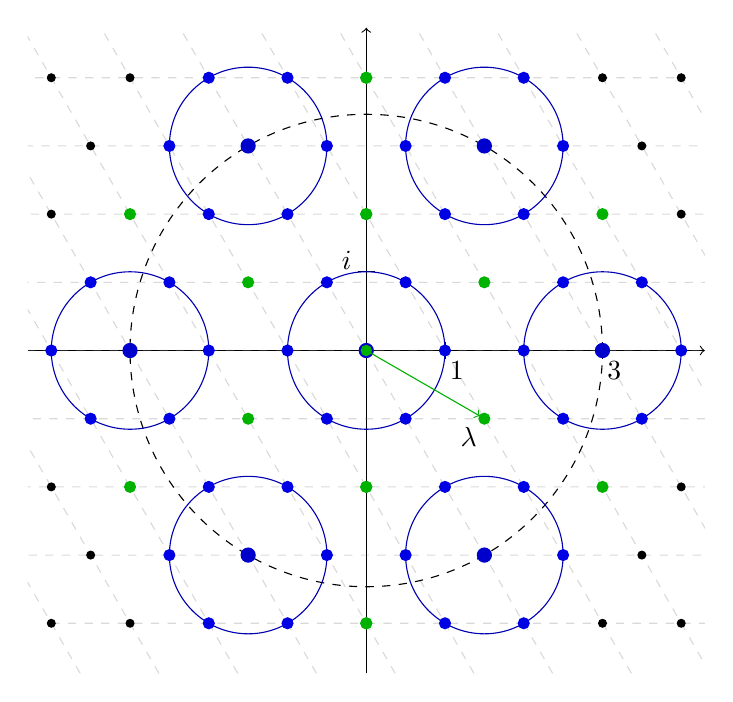
\begin{tikzpicture}
				\clip (-4.3, -4.1) rectangle (4.3, 4.1);
				\draw [->] (-4.3, 0) -- (4.3, 0);
				\draw [->] (0, -4.1) -- (0, 4.1);
				
				\draw (1,3pt) -- (1,-3pt);
				\draw (3pt,1) -- (-3pt,1);
				\draw (3,3pt) -- (3,-3pt);
				
				\pgftransformcm{1}{0}{-1/2}{1.7320501/2}{\pgfpoint{0cm}{0cm}}
				\draw[style=help lines,dashed, thin, gray, opacity=0.3] (-6,-6) grid (6,6);
				\pgftransformcm{1}{0}{1/1.7320501}{2/1.7320501}{\pgfpoint{0cm}{0cm}}
				
				\node at (1.15, -0.25) {$1$};
				\node at (3.15, -0.25) {$3$};
				\node at (-0.25, 1.15) {$i$};
				
				\def\aa{-1/2};
				\def\bb{1.7320501/2};
				
				\foreach \x in {-6, -5, ..., 6}{
					\foreach \y in {-6, -5, ..., 6}{
						\node[draw,circle,inner sep=1pt,fill] at (\x + \y* \aa, \y * \bb) {};
					}
				}
			
				\draw[black, dashed] (0, 0) circle[radius=3];
				
				\foreach \x/\y in {0/0, 1.5/{3 * \bb}, 3/0, -3/0, -1.5/{3 * \bb}, -1.5/{-3 * \bb}, 1.5/{-3 * \bb}}{
					\draw[black!30!blue] (\x, \y) circle[radius=1];
					\node[draw,circle,inner sep=1.8pt,fill,black!20!blue] at (\x, \y) {};
					\node[draw,circle,inner sep=1.4pt,fill,black!10!blue] at ({\x - 1/2}, {\y + \bb}) {};
					\node[draw,circle,inner sep=1.4pt,fill,black!10!blue] at ({\x + 1/2}, {\y + \bb}) {};
					\node[draw,circle,inner sep=1.4pt,fill,black!10!blue] at ({\x + 1}, \y) {};
					\node[draw,circle,inner sep=1.4pt,fill,black!10!blue] at ({\x - 1}, \y) {};
					\node[draw,circle,inner sep=1.4pt,fill,black!10!blue] at ({\x + 1/2}, {\y - \bb}) {};
					\node[draw,circle,inner sep=1.4pt,fill,black!10!blue] at ({\x - 1/2}, {\y - \bb}) {};
				}
				
				\node[draw,circle,inner sep=1.3pt,fill,black!30!green] at (0, 0) {};
				\foreach \x in {-2, -1, 1, 2}{
					\node[draw,circle,inner sep=1.4pt,fill,black!30!green] at (1.5 * \x, -\bb  * \x) {};
					\node[draw,circle,inner sep=1.4pt,fill,black!30!green] at (1.5 * \x, \bb  * \x) {};
					\node[draw,circle,inner sep=1.4pt,fill,black!30!green] at (0, -2 * \bb  * \x) {};
					\node[draw,circle,inner sep=1.4pt,fill,black!30!green] at (0, 2 * \bb  * \x) {};
				}
				
				\draw [->, black!30!green] (0, 0) -- (1.5 - 0.055, -\bb + 0.033) node [black, below left, scale = 1] {};
				\node at (1.5 - 0.2, -\bb - 0.23) {$\lambda$};
			\end{tikzpicture}
		}
	\end{center}
	
	Таким образом, $z = 3u + r$, тогда $z^3 \equiv_9 r^3 = \pm 1$.
\end{proof}

\begin{corollary}
	Если $\pm x^3 \pm y^3 \pm z^3 = 0$ для некоторых $x, y, z \in \Z[\omega]$, то $\lambda \mid xyz$.
\end{corollary}

\begin{proof}
	Если это не так, то $0 = \pm x^3 \pm y^3 \pm z^3 \equiv_9 \pm 1$ --- противоречие.
\end{proof}

\begin{corollary}
	Если $r_xx^3 + r_xy^3 = r_zz^3\lambda^{3k}$ для некоторых $x, y, z \in \Z[\omega]$, $r_x, r_y, r_z \in \Z[\omega]^*$, $k \in \N$, причем $\lambda \nmid xyz$, то выполнено следующее:
	\begin{enumerate}
		\item $k \ge 2$
		\item $r_x = \pm r_y$
	\end{enumerate}
\end{corollary}

\begin{proof}
	Рассмотрим равенство из условия по модулю 9: $\pm r_x \pm r_y \equiv_9 \pm r_z\lambda^{3k}$. Если $k = 1$, то $0 \le N(\pm r_x \pm r_y) \le 2 < N(r_z\lambda^{3})< 9$, поэтому данное сравнение не может быть выполнено. Если же $k \ge 2$, то правая часть делится на 9, поэтому $\pm r_x \pm r_y = 0$, откуда $r_x = \pm r_y$.
\end{proof}

\begin{theorem}[Великая теорема Ферма при $n = 3$]
	Уравнение $x^3 + y^3 = z^3$ не имеет нетривиальных целочисленных решений.
\end{theorem}

\begin{proof}
	Достаточно показать, что равенство $x^3 + y^3 = rz^3\lambda^{3k}$ не может быть выполнено ни для каких попарно взаимно простых $x, y, z \in \Z[\omega]$, $r \in \Z[\omega]^*$, $k \in \N$, $\lambda \nmid xyz$.
	
	Предположим, что это не так. Выберем такой набор чисел, удовлетворяющих равенству, в котором число $k$ минимально. Тогда, как уже было доказано, $k \ge 2$. Перепишем равенство в виде $(x + y)(x + \omega y)(x + \omega^2 y) = rz^3\lambda^{3k}$. Заметим, что $(x + y, x + \omega y) = (x + y, \lambda y)$, $x + y = (x + \omega y) + \lambda y$ и $x + y = (x + \omega^2 y) + \lambda (1 + \omega) y$, поэтому числа $x + y, x + \omega y, x + \omega^2 y$ имеют единственный общий делитель $\lambda$. Значит, без ограничения общности их можно представить в следующем виде:
	\begin{align*}
		x + y &= r_x x_0^3 \lambda, r_x \in \Z[\omega]^*, x_0 \in \Z[\omega]\\
		x + \omega y &= r_y y_0^3 \lambda, r_y \in \Z[\omega]^*, y_0 \in \Z[\omega]\\
		x + \omega^2y &= r_z z_0^3 \lambda^{3k - 2}, r_z \in \Z[\omega]^*, z_0 \in \Z[\omega]
	\end{align*}
	
	Но тогда, поскольку $(x + y) + \omega(x + \omega y) + \omega^2(x + \omega^2 y) = 0$, выполнено следующее:
	\[r_x x_0^3 + (r_y\omega) y_0^3 + (r_z \omega^2) z_0^3 \lambda^{3(k - 1)} = 0\]
	
	Тогда, как уже было доказано, $r_x = \pm r_y \omega$, поэтому получен набор чисел, удовлетворяющий равенству, с меньшим показателем степени у $\lambda$ --- противоречие.
\end{proof}